% 本模板根据中国科学院大学本科生公共必修课程《基础物理实验》Word模板格式编写
% 本模板由Shing-Ho Lin和Jun-Xiong Ji于2022年9月共同完成, 旨在方便LaTeX原教旨主义者和被Word迫害者写实验报告, 避免Word文档因插入过多图与公式造成卡顿. 
% 如有任何问题, 请联系: linchenghao21@mails.ucas.ac.cn
% This is the LaTeX template for experiment report of Experimental Physics courses, based on its provided Word template. 
% This template is completed by the joint collabration of Shing-Ho Lin and Junxiong Ji in September 2022. 
% Adding numerous pictures and equations leads to unsatisfying experience in Word. Therefore LaTeX is better. 
% Feel free to contact us via: linchenghao21@mails.ucas.ac.cn

\documentclass[11pt]{article}

\usepackage[a4paper]{geometry}
\geometry{left=2.0cm,right=2.0cm,top=2.5cm,bottom=2.5cm}

\usepackage{ctex} % 支持中文的LaTeX宏包
\usepackage{amsmath,amsfonts,graphicx,subfigure,amssymb,bm,amsthm,mathrsfs,mathtools,breqn} % 数学公式和符号的宏包集合
\usepackage{algorithm,algorithmicx} % 算法和伪代码的宏包
\usepackage[noend]{algpseudocode} % 算法和伪代码的宏包
\usepackage{fancyhdr} % 自定义页眉页脚的宏包
\usepackage[framemethod=TikZ]{mdframed} % 创建带边框的框架的宏包
\usepackage{fontspec} % 字体设置的宏包
\usepackage{adjustbox} % 调整盒子大小的宏包
\usepackage{fontsize} % 设置字体大小的宏包
\usepackage{tikz,xcolor} % 绘制图形和使用颜色的宏包
\usepackage{multicol} % 多栏排版的宏包
\usepackage{multirow} % 表格中合并单元格的宏包
\usepackage{pdfpages} % 插入PDF文件的宏包
\RequirePackage{listings} % 在文档中插入源代码的宏包
\RequirePackage{xcolor} % 定义和使用颜色的宏包
\usepackage{wrapfig} % 文字绕排图片的宏包
\usepackage{bigstrut,multirow,rotating} % 支持在表格中使用特殊命令的宏包
\usepackage{booktabs} % 创建美观的表格的宏包
\usepackage{circuitikz} % 绘制电路图的宏包

\definecolor{dkgreen}{rgb}{0,0.6,0}
\definecolor{gray}{rgb}{0.5,0.5,0.5}
\definecolor{mauve}{rgb}{0.58,0,0.82}
\lstset{
  frame=tb,
  aboveskip=3mm,
  belowskip=3mm,
  showstringspaces=false,
  columns=flexible,
  framerule=1pt,
  rulecolor=\color{gray!35},
  backgroundcolor=\color{gray!5},
  basicstyle={\small\ttfamily},
  numbers=none,
  numberstyle=\tiny\color{gray},
  keywordstyle=\color{blue},
  commentstyle=\color{dkgreen},
  stringstyle=\color{mauve},
  breaklines=true,
  breakatwhitespace=true,
  tabsize=3,
}

% 轻松引用, 可以用\cref{}指令直接引用, 自动加前缀. 
% 例: 图片label为fig:1
% \cref{fig:1} => Figure.1
% \ref{fig:1}  => 1
\usepackage[capitalize]{cleveref}
% \crefname{section}{Sec.}{Secs.}
\Crefname{section}{Section}{Sections}
\Crefname{table}{Table}{Tables}
\crefname{table}{Table.}{Tabs.}

\setmainfont{Palatino Linotype.ttf}
\setCJKmainfont{SimHei.ttf}
% \setCJKsansfont{Songti.ttf}
% \setCJKmonofont{SimSun.ttf}
\punctstyle{kaiming}
% 偏好的几个字体, 可以根据需要自行加入字体ttf文件并调用

\renewcommand{\emph}[1]{\begin{kaishu}#1\end{kaishu}}

%改这里可以修改实验报告表头的信息
\newcommand{\experiName}{气垫导轨实验}
\newcommand{\supervisor}{姚楚豪}
\newcommand{\name}{张欣培}
\newcommand{\studentNum}{2022K8009922001}
\newcommand{\class}{01}
\newcommand{\group}{10}
\newcommand{\seat}{9}
\newcommand{\dateYear}{2023}
\newcommand{\dateMonth}{10}
\newcommand{\dateDay}{23}
\newcommand{\room}{教716}
\newcommand{\others}{$\square$}
%% 如果是调课、补课, 改为: $\square$\hspace{-1em}$\surd$
%% 否则, 请用: $\square$
%%%%%%%%%%%%%%%%%%%%%%%%%%%

\begin{document}

%若需在页眉部分加入内容, 可以在这里输入
% \pagestyle{fancy}
% \lhead{\kaishu 测试}
% \chead{}
% \rhead{}

\begin{center}
    \LARGE \bf 《\, 基\, 础\, 物\, 理\, 实\, 验\, 》\, 实\, 验\, 报\, 告
\end{center}

\begin{center}
    \noindent \emph{实验名称}\underline{\makebox[25em][c]{\experiName}}
    \emph{指导教师}\underline{\makebox[8em][c]{\supervisor}}\\
    \emph{姓名}\underline{\makebox[6em][c]{\name}} 
    % 如果名字比较长, 可以修改box的长度"6em"
    \emph{学号}\underline{\makebox[10em][c]{\studentNum}}
    \emph{分班分组及座号} \underline{\makebox[5em][c]{\class \ -\ \group \ -\ \seat }\emph{号}} (\emph{例}:\, 1\,-\,04\,-\,5\emph{号})\\
    \emph{实验日期} \underline{\makebox[3em][c]{\dateYear}}\emph{年}
    \underline{\makebox[2em][c]{\dateMonth}}\emph{月}
    \underline{\makebox[2em][c]{\dateDay}}\emph{日}
    \emph{实验地点}\underline{{\makebox[4em][c]\room}}
    \emph{调课/补课} \underline{\makebox[3em][c]{\others\ 是}}
    \emph{成绩评定} \underline{\hspace{5em}}
    {\noindent}
    \rule[8pt]{17cm}{0.2em}
\end{center}

\begin{center}
    \Large \bf 第一部分\qquad 实验内容
\end{center}

\section{实验目的}

\begin{enumerate}
    \item 了解气垫导轨和数字毫秒计的使用方法
    \item 观察并测量简谐运动相关物理量
    \item 验证机械能守恒定律(弹性势能与动能相互转换)
    \item 深入了解平均速度和瞬时速度的关系,用极限法测定瞬时速度
    \item 测定弹簧的劲度系数,以验证胡克定律/检验弹簧是否良好
\end{enumerate}

\section{实验器材}

    气垫导轨,数字毫秒计,数字天平,滑块,配重物,挡光片(U型,平板),光电门等。

\section{实验原理}
\begin{enumerate}
    \item 简谐运动 \newline \hspace*{2em} 简谐运动是指物体在某一平衡位置附近作往复运动,其加速度与位移成正比,与位移方向相反,且加速度的大小与位移成正比。简谐运动的物体称为振动体,振动体的运动轨迹称为振动轨迹。简谐运动的物体在平衡位置附近的运动可以用简谐运动的基本方程来描述:$x=A\sin(\omega t+\varphi_0)$,其中A为振幅,$\omega$为角频率,$\varphi_0$为初相位。
    \item 弹簧与胡克定律 \newline \hspace*{2em} 对于弹簧振子,由胡克定律,其受力$F=-kx$,受到的加速度为$a=-\frac{k}{m}x$,其中k为弹簧劲度系数,m为振子质量。由此可得到振子的运动方程为$\frac{d^2x}{dt^2}+\frac{k}{m}x=0$,解得$x=A\sin(\omega t+\varphi_0)$,其中$\omega=\sqrt{\frac{k}{m}}$,A为振幅,$\varphi_0$为初相位。于是,弹簧振子的运动为简谐振动。
    \item 机械能守恒 \newline \hspace*{2em} 机械能守恒的内容为:只有在重力(或弹簧的弹力)做功的情形下,物体的重力势能(或弹性势能)和动能发生相互转化,但总机械能保持不变。本实验中,保持气垫导轨水平,不产生重力做功,在忽略阻力的情况下,仅有弹簧弹力做功,因此机械能守恒成立。考虑阻力微弱影响后,机械能守恒也应近似成立。
    \item 平均速度与瞬时速度 \newline \hspace*{2em} 瞬时速度的定义为$v=\frac{dx}{dt}$。我们无法测量时间无穷小时物体的位移。我们能够测量物体通过一小段位移所用时间,进而求出通过此段的平均速度$\bar{v}=\frac{\Delta x}{\Delta t}$。当时间足够小时,极限$\lim\limits_{\Delta t \to 0^{+}}\frac{\Delta x}{\Delta t}$就是瞬时速度。
\end{enumerate}


\section{实验内容}
    由于测定瞬时速度实验无需调平气垫导轨,先进行此实验。然后进行调平气垫导轨。测定弹簧的劲度系数实验能够检验弹簧是否良好,次之。
\subsection {测定瞬时速度}
对应数据表实验八、九、十。
\begin{enumerate}
    \item 实验步骤
    \begin{enumerate}
        \item 打开气泵开关,加入垫块调整气垫导轨至倾斜状态。打开数字毫秒计,调整至测速模式。滑块上安装U型挡光片(1cm、3cm、5cm、10cm)。
        \item 将滑块放置在气垫导轨上,使其静止。调整光电门位置,使其中间位置与U型挡光片最前端位置的距离为50cm(AP距离50cm)。
        \item 释放滑块,读取数字毫秒计显示的速度值。记录数据。
        \item 重复c)四次,记录数据。
        \item 改变U型挡光片的长度,重复b)-d)。(实验八)
        \item 改变气垫导轨倾斜角度,重复b)-e)。(实验九)
        \item 调整光电门位置,使其中间位置与U型挡光片最前端位置的距离为60cm(AP距离60cm)。重复c)-e)。(实验十)
        \item 整理器材。
    \end{enumerate}
    \item 实验数据
        
        \begin{table}[H]
          \centering
          \caption{测定瞬时速度}
            \begin{tabular}{|r|r|r|r|r|r|r|}\hline
            挡光片长度/$cm$ & $\bar{\Delta t_{1}}/ms$ & $\bar{\Delta t_{2}}/ms$ & $\bar{\Delta t_{3}}/ms$ & $\bar{\Delta v_{1}}/(cm \cdot s^{-1})$ & $\bar{\Delta v_{2}}/(cm \cdot s^{-1})$ & $\bar{\Delta v_{3}}/(cm \cdot s^{-1})$ \\\hline
            1    & 29.49  & 20.75  & 26.81  & 33.91  & 48.19  & 37.30  \\\hline
            3    & 86.84  & 62.02  & 80.08  & 34.55  & 48.37  & 37.46  \\\hline
            5    & 145.18  & 102.08  & 131.64  & 34.44  & 48.98  & 37.98  \\\hline
            10   & 283.20  & 199.73  & 258.38  & 35.31  & 50.07  & 38.70  \\\hline
            \end{tabular}%
          \label{tab:瞬时速度}%
        \end{table}%
        
        \begin{figure}[H]
            \begin{minipage}[t]{0.49\linewidth}
                \centering
                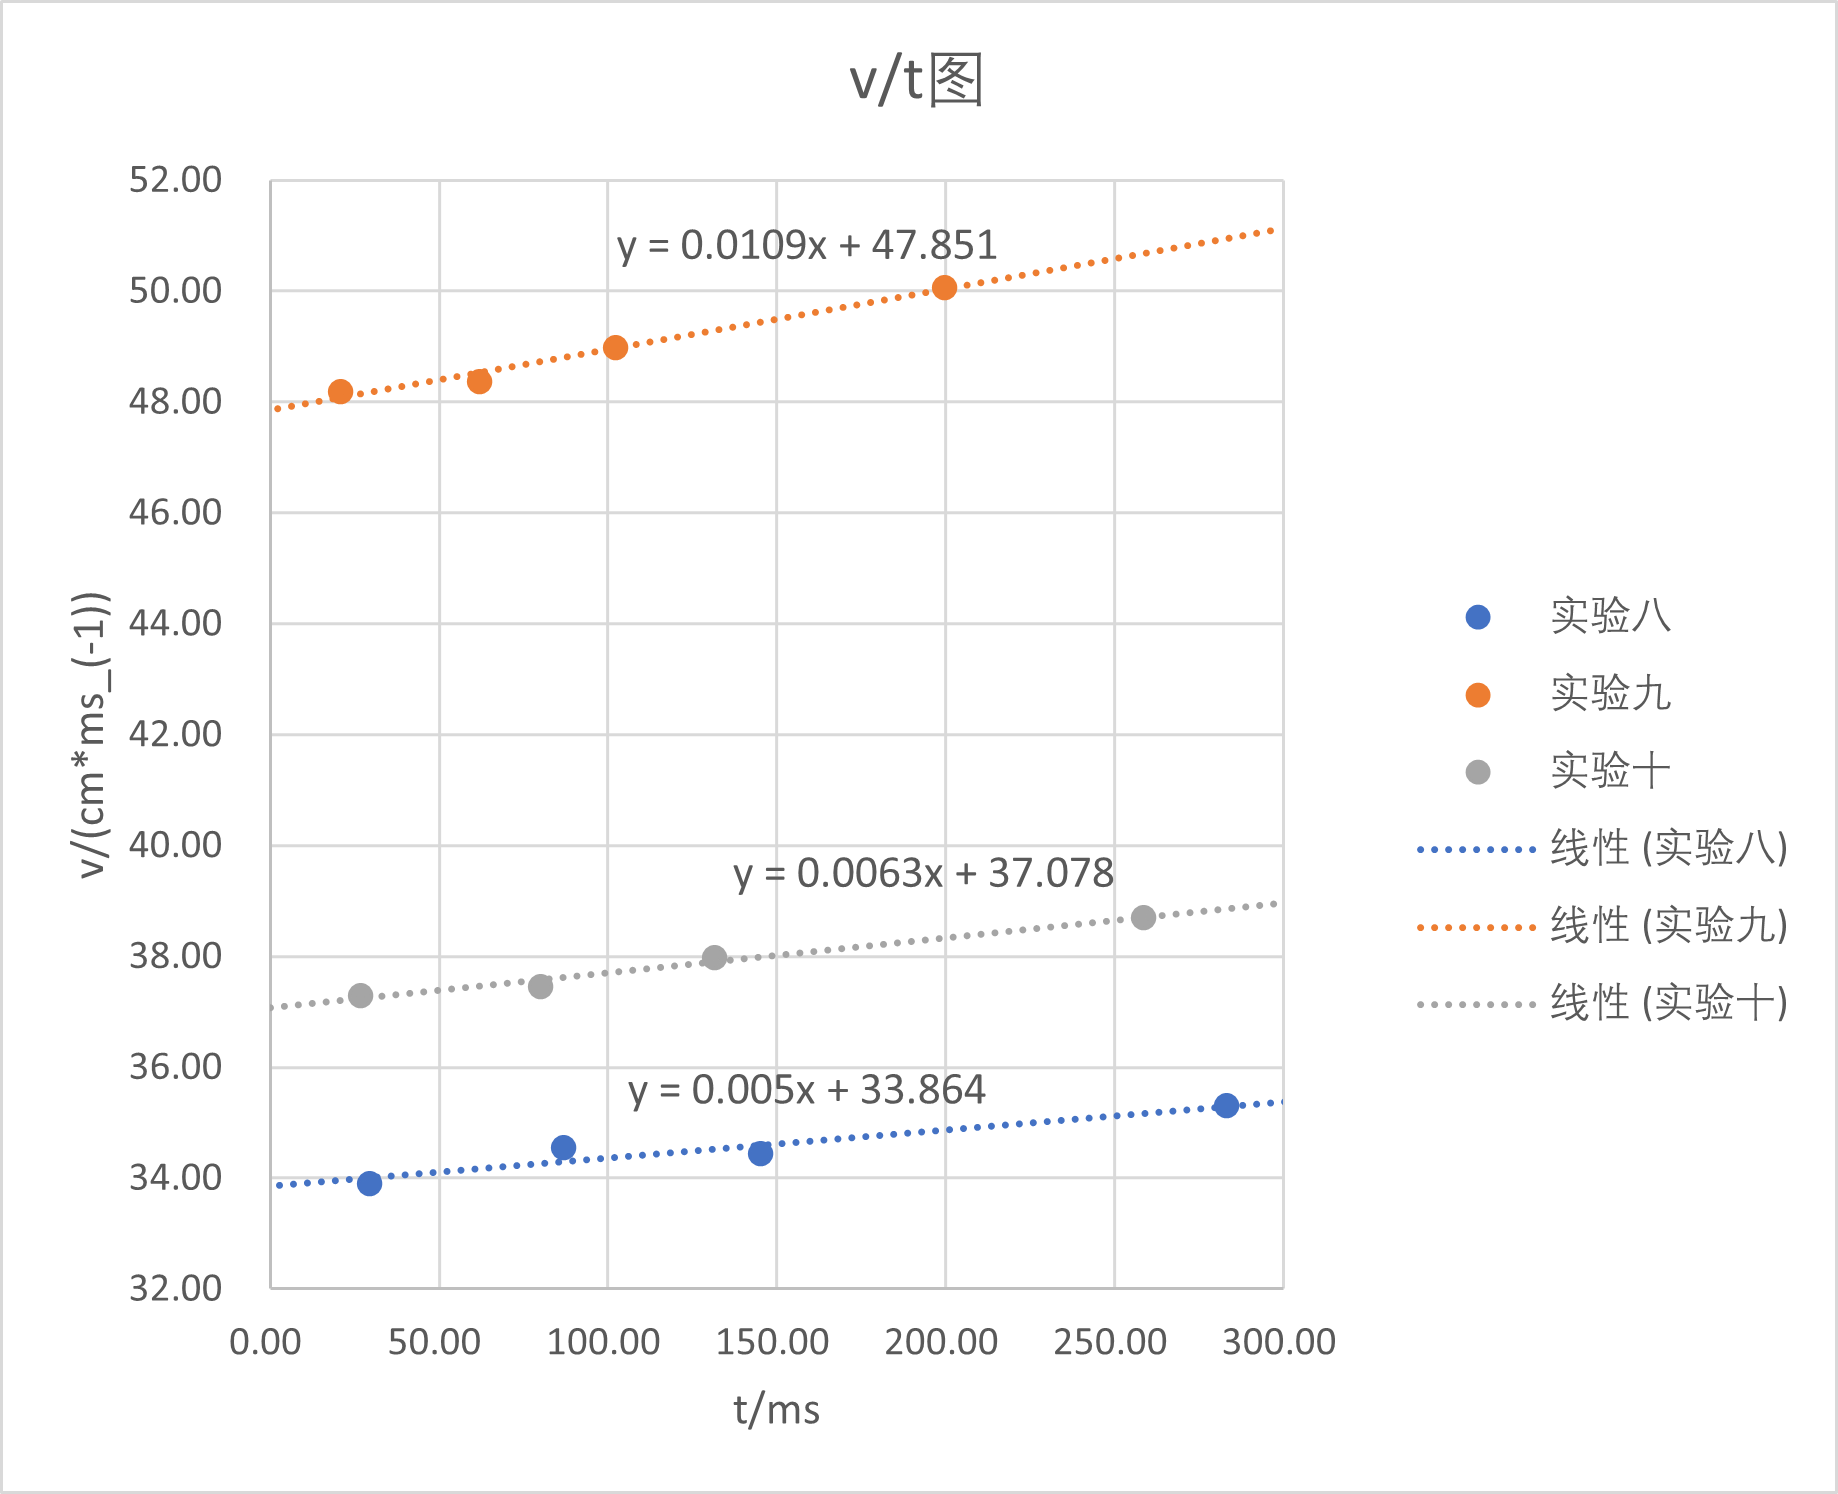
\includegraphics[width=8cm]{Fig/瞬时速度vt.png}
                \caption{测定瞬时速度v-t图}
            \end{minipage}
            \begin{minipage}[t]{0.49\linewidth}
                \centering
                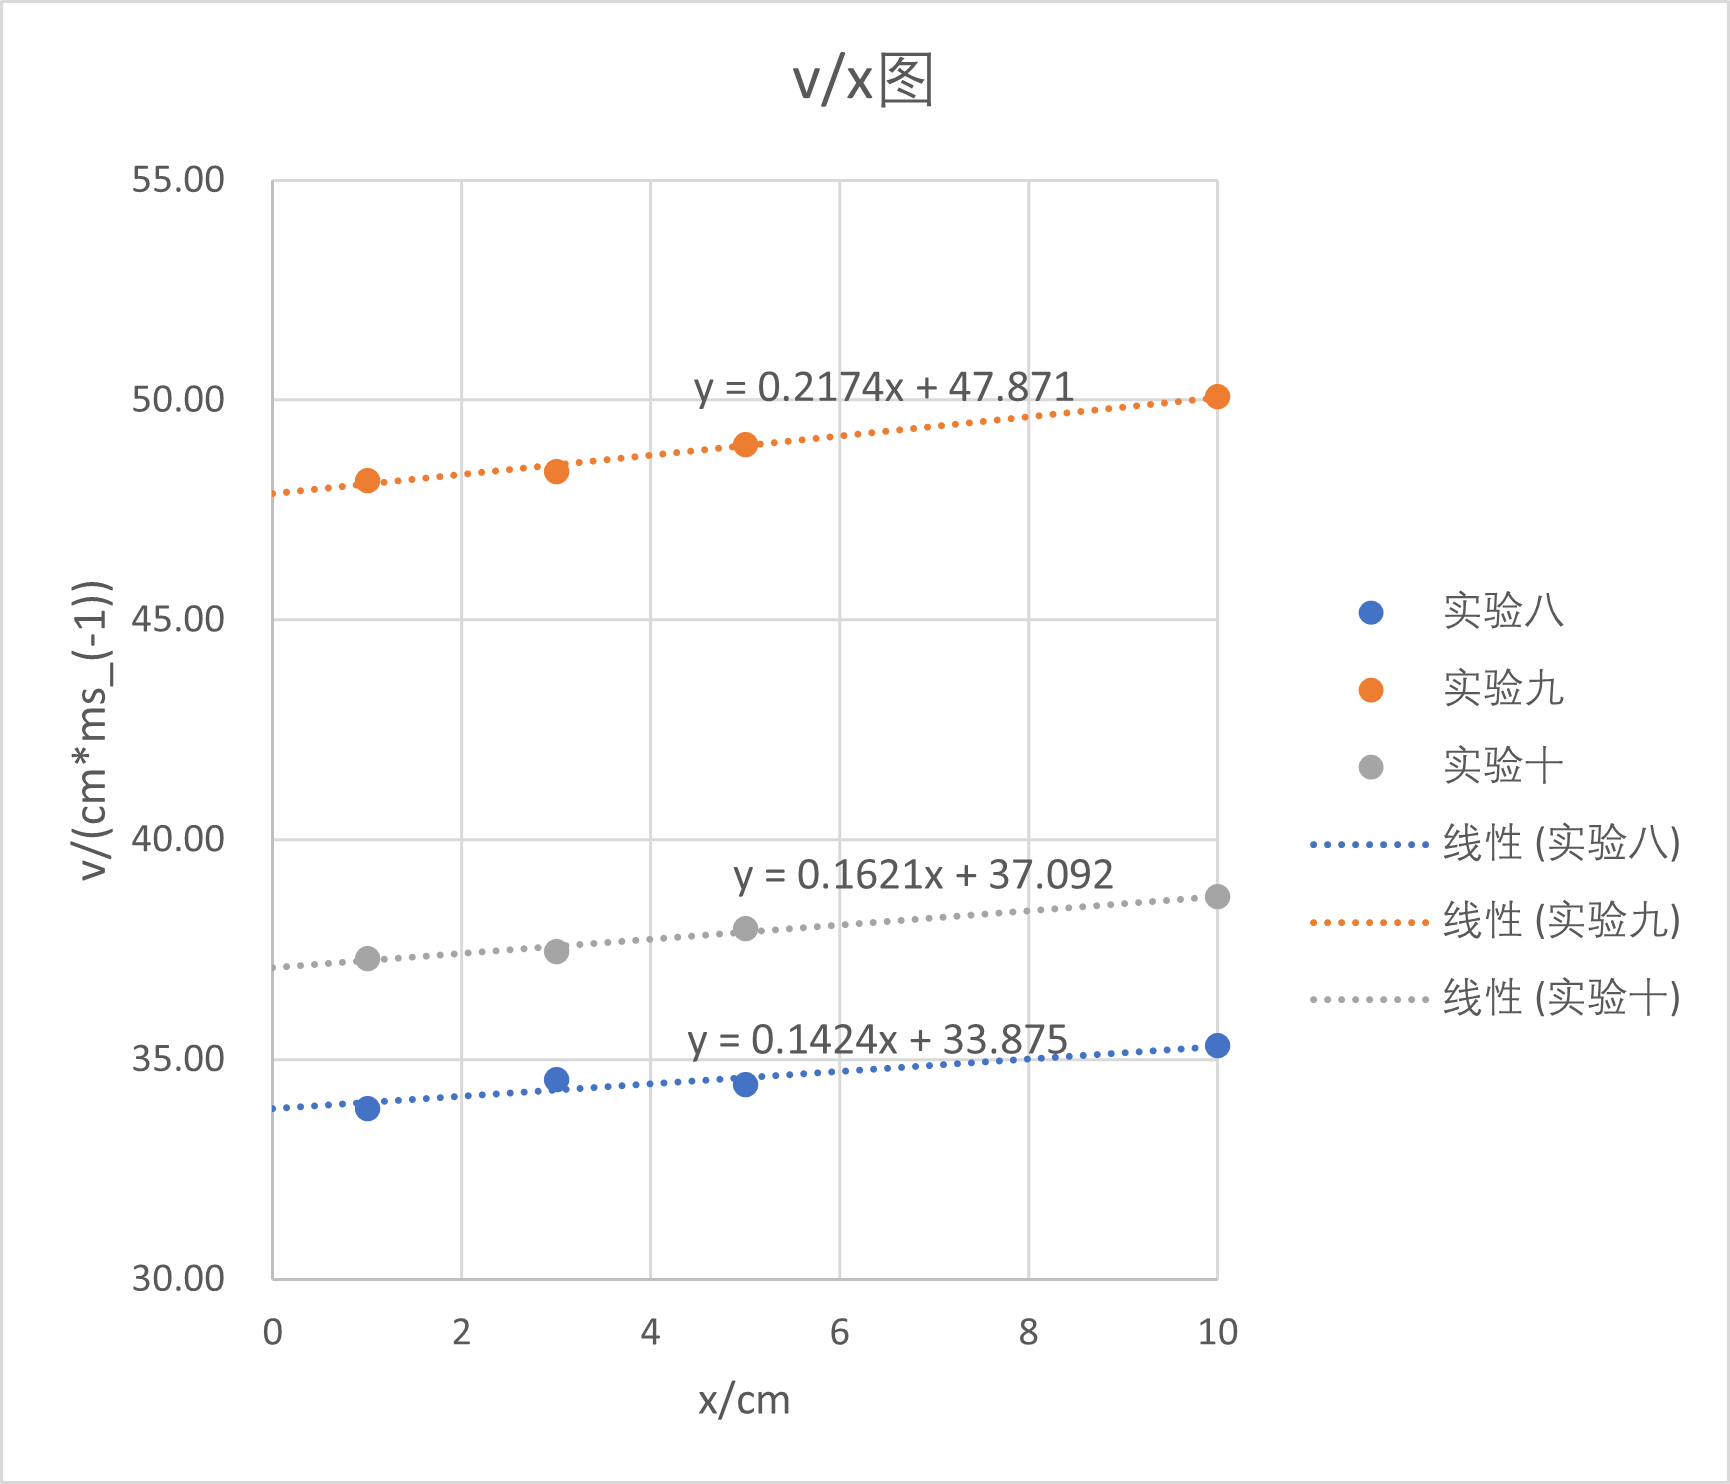
\includegraphics[width=8cm]{Fig/瞬时速度vx.png}
                \caption{测定瞬时速度v-x图}
            \end{minipage}
        \end{figure} 
    \item 数据分析
    \begin{enumerate}
        \item 由$\bar{\Delta v}=\frac{\Delta x}{\Delta t}=v_{0}+\frac{a}{2} \Delta t$,根据上图数据拟合,截距即为瞬时速度,斜率即为加速度的二分之一。将速度保留一位小数,$\bar{\Delta v_{1}}=33.9(cm \cdot s^{-1})$,$\bar{\Delta v_{2}}=37.1(cm \cdot s^{-1})$,$\bar{\Delta v_{3}}=47.9(cm \cdot s^{-1})$。在此精度下,$v-t$和$v-x$图所得数据一致。
        \item 表格中,3cm和5cm时的$\bar{\Delta v_{1}}$数据反常,5cm的平均速度理应大于3cm时,这会造成误差。
        \item 实验时,实验八和实验十我将气垫导轨用两个垫块垫高,理论上倾斜角度相同时滑块受到的加速度应该相同,但是所得出的加速度不同。可能是因为挪动气垫导轨导致实际的气垫导轨倾斜角度并不相同。
    \end{enumerate}
    
\end{enumerate}
\subsection{调平气垫导轨}
对应数据表实验一
\begin{enumerate}
    \item 实验步骤
    \begin{enumerate}
        \item 打开气泵开关,加入垫块调整气垫导轨至倾斜状态。打开数字毫秒计,调整至测速模式。滑块上安装U型挡光片(1cm)。在气垫导轨两个位置安装光电门,保证两光电门距离不过近。
        \item 轻推滑块使其通过两光电门,对两次通过光电门的速度进行读数,根据读数调整气垫导轨水平。
        \item 重复b)多次,直至两次通过光电门速度接近,偏差小于千分之五。
    \end{enumerate}
    \item 实验数据
    % Table generated by Excel2LaTeX from sheet 'Sheet1'
        \begin{table}[H]
          \centering
          \caption{调整气垫导轨水平}
            \begin{tabular}{|r|r|r|}\hline
            $v_{1}/(cm \cdot s^{-1})$ & $v_{2}/(cm \cdot s^{-1})$ & 误差/\% \\\hline
            24.09 & 23.95 & 0.58 \\\hline
            34.09 & 33.97 & 0.35 \\\hline
            40.06 & 39.89 & 0.42 \\\hline
            \end{tabular}%
          \label{tab:addlabel}%
        \end{table}%
\end{enumerate}
此次调平后,后续实验不再重复调平步骤。

\subsection{测量弹簧振子的振动周期并考察振动周期和振幅的关系}
对应数据表实验二
\begin{enumerate}
    \item 实验步骤
    \begin{enumerate}
        \item 将条形挡光片安装在滑块上。连接设备,将滑块两端用弹簧连接,放在气垫导轨上。在接近滑块平衡位置的地方安装一个光电门。将数字毫秒计调整至周期模式。
        \item 将滑块拉至距离平衡位置10cm处,释放滑块,等待五个周期,读取数字毫秒计显示的五个周期值并取平均。
        \item 重复b),改变滑块初始释放位置为距离平衡位置(20,30,40)cm。
    \end{enumerate}
    \item 实验数据
    % Table generated by Excel2LaTeX from sheet 'Sheet1'
        \begin{table}[H]
          \centering
          \caption{振动周期和振幅的关系}
            \begin{tabular}{|l|r|r|r|r|}\hline 
                   & 10cm & 20cm & 30cm & 40cm \\\hline
            $t/ms$  & 1504.53 & 1503.39 & 1503.51 & 1503.5 \\\hline
            \end{tabular}%
          \label{tab:addlabel}%
        \end{table}%
    \item 数据分析
    \begin{enumerate}
        \item 振子的振动周期在$1504ms\pm 0.7ms$范围内,与振幅无关。
    \end{enumerate}
\end{enumerate}

\subsection{研究振动周期和振子质量之间的关系}
对应数据表实验三
\begin{enumerate}
    \item 实验步骤
    \begin{enumerate}
        \item 用数字天平测配重物质量。
        \item 将条形挡光片安装在滑块上。连接设备,将滑块两端用弹簧连接,放在气垫导轨上。在接近滑块平衡位置的地方安装一个光电门。将数字毫秒计调整至周期模式。
        \item 将滑块拉至距离平衡位置40cm处,释放滑块,等待十个周期,读取数字毫秒计显示的十个周期值并取平均。
        \item 改变滑块上的配重物质量,重复c,再进行四次实验。
    \end{enumerate}
    \item 实验数据
    \newline 滑块质量216.32g,条型挡光片质量2.21g,两者之和$m_{1}=218.53g$。
    % Table generated by Excel2LaTeX from sheet 'Sheet1'
        \begin{table}[H]
          \centering
          \caption{振动周期和振子质量}
            \begin{tabular}{|l|r|r|r|r|r|}\hline
            
                配重物质量$m/g$    & 0.00   & 12.39  & 25.01  & 37.40  & 50.00  \\\hline
                振子总质量$m_{1}/g$ & 218.53  & 230.92  & 243.54  & 255.93  & 268.53  \\\hline
                $t/ms$   & 1503.23  & 1544.86  & 1585.65  & 1624.70  & 1663.57  \\\hline
                $t^{2}/s$ & 2.260  & 2.387  & 2.514  & 2.640  & 2.767  \\\hline
    
            \end{tabular}%
          \label{tab:振动周期和振子质量}%
        \end{table}%
        \begin{figure}[H]
            \centering
            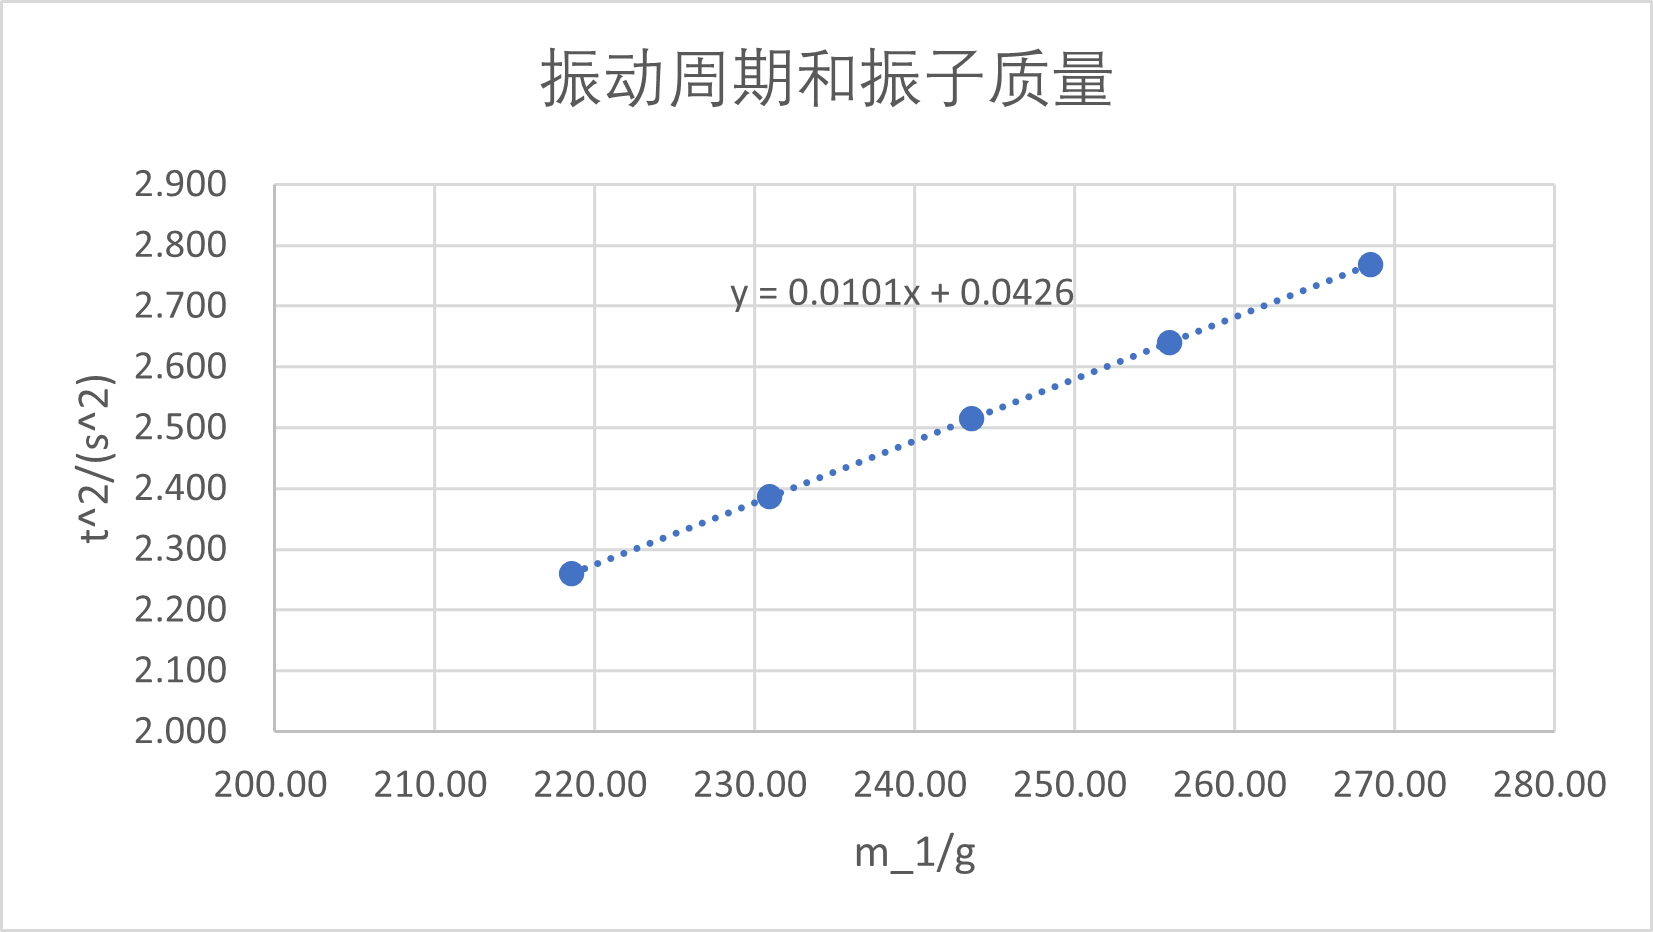
\includegraphics[width=12cm]{Fig/振动周期和振子质量.png}
            \caption{振动周期和振子质量$t^{2}/m_{1}$图}
        \end{figure}
    \item 数据分析
    \begin{enumerate}
        \item 上图斜率$a=0.0101$,截距$b=0.0426$
        \item 由$T^{2}=\frac{4\pi^{2}(m_{1}+m_{0})}{k}$,设$m_{1}$为振子总质量,$m_{0}$为弹簧有效质量。于是有$a=\frac{4\pi^{2}}{k}$,$k=\frac{4\pi^{2}}{a}=3909(g/s^{2})=3.909(N \cdot s)$。图像截距为$b=\frac{4\pi^{2}m_{0}}{k}$,得弹簧等效质量$m_{0}=b \cdot \frac{k}{4\pi^{2}}=4.22g$。
    \end{enumerate}
\end{enumerate}

\subsection{研究速度和位移的关系}
对应数据表实验四
\begin{enumerate}
    \item 实验步骤
    \begin{enumerate}
        \item 将U形挡光片(1cm)安装在滑块上。连接设备,将滑块两端用弹簧连接,放在气垫导轨上。将数字毫秒计调整至测速模式。
        \item 将光电门移动至距离滑块平衡位置10cm处,将滑块拉至距离平衡位置40cm处,释放滑块,测滑块经过光电门的速度,记录数字毫秒计读数。
        \item 重复b)两次,取平均值。
        \item 改变光电门移动至距离滑块平衡位置为(15,20,25,30)cm,重复b)c),再进行四次实验。
    \end{enumerate}
    \item 实验数据
    \newline 滑块质量216.32g,U型挡光片质量11.72g,弹簧等效质量两者之和4.22g,三者之和$m=232.26g$。振幅40cm。
    \newline 由能量守恒,$\frac{1}{2}kx^{2}+\frac{1}{2}mv^{2}=\frac{1}{2}kA^2$,得计算值$v=\sqrt{\frac{k}{m}} \sqrt{A^{2}-x^{2}}$。
    % Table generated by Excel2LaTeX from sheet 'Sheet1'
        \begin{table}[H]
          \centering
          \caption{速度和位移}
            \begin{tabular}{|l|r|r|r|r|r|}\hline
            $x/cm$   & 10     & 15     & 20     & 25     & 30 \\\hline
            $v/(cm \cdot s^{-1})$ & 157.07  & 150.00  & 139.99  & 125.94  & 105.52  \\\hline
            计算值$v/(cm \cdot s^{-1})$ & 158.79  & 152.03  & 142.03  & 128.02  & 108.48  \\\hline
            \end{tabular}%
          \label{tab:速度和位移}%
        \end{table}%
        \begin{figure}[H]
            \centering
            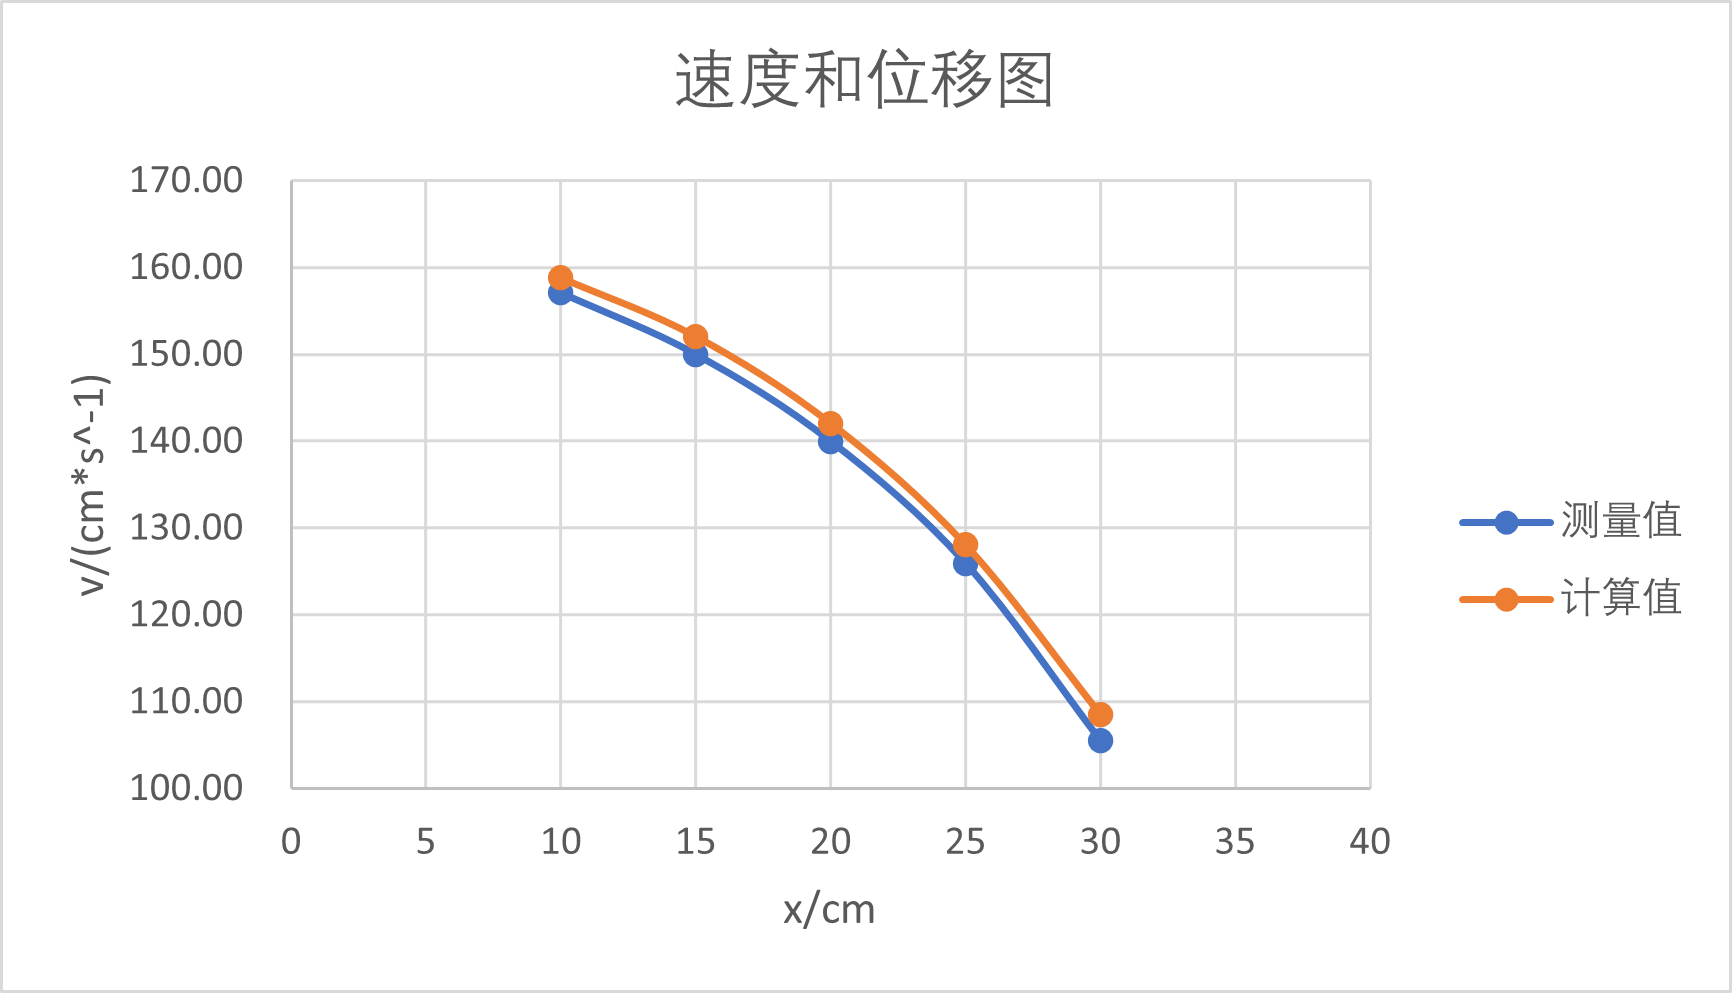
\includegraphics[width=12cm]{Fig/速度和位移.png}
            \caption{速度和位移$v/x$图}
        \end{figure}
    \item 数据分析
    \begin{enumerate}
        \item 我们发现,计算值与测量值基本贴近,误差在$3cm/s$以内,测量值均小于计算值。可能的原因是
        \newline (1)气垫导轨微小阻力导致滑块速度减小
        \newline (2)弹簧等效质量不为常数,是和滑块质量相关的变量。原因是,滑块质量越大,气膜对其支撑越差,滑块下降,增加弹簧等效质量。
        \newline (3)释放滑块时,滑块与轨道产生短时间摩擦,发生能量损耗。
    \end{enumerate}
\end{enumerate}

\subsection{研究振动系统的机械能是否守恒}
对应数据表实验五
\begin{enumerate}
    \item 实验数据
    \newline 数据来源于4.5
    % Table generated by Excel2LaTeX from sheet 'Sheet1'
        \begin{table}[H]
          \centering
          \caption{振动系统的机械能}
            \begin{tabular}{|l|r|r|r|r|r|}\hline
                $v/(cm \cdot s^{-1})$ & 157.07  & 150.00  & 139.99  & 125.94  & 105.52  \\\hline
                $E_{k}/J$     & 0.2865  & 0.2613  & 0.2276  & 0.1842  & 0.1293  \\\hline
                $E_{p}/J$     & 0.0195  & 0.0440  & 0.0782  & 0.1222  & 0.1759  \\\hline
                $E/J$      & 0.3060  & 0.3053  & 0.3058  & 0.3063  & 0.3052  \\\hline

            \end{tabular}%
          \label{tab:振动系统的机械能}%
        \end{table}%
    \item 数据分析
    \begin{enumerate}
        \item $E=0.3057J \pm 0.0006J$在保留两位有效数字的情况下,$E=0.31J$。在不考虑阻力影响的情况下,满足机械能守恒。
    \end{enumerate}

\end{enumerate}

\subsection{测定弹簧的劲度系数}
对应数据表实验六
\begin{enumerate}
    \item 实验步骤
    \begin{enumerate}
        \item 将U型挡光片(1cm)安装在滑块上。连接设备,将滑块两端用弹簧连接,放在气垫导轨上。在接近滑块平衡位置的地方安装一个光电门。将数字毫秒计调整至测速模式。
        \item 将滑块拉至距离平衡位置10cm处,释放滑块,读取数字毫秒计显示的速度值。
        \item 重复b)再测量两组数据,取平均值。
        \item 重复b)c),改变滑块初始释放位置为距离平衡位置(15,20,25,30)cm处,进行多次实验。
    \end{enumerate}
    \item 实验数据
    % Table generated by Excel2LaTeX from sheet 'Sheet1'
        \begin{table}[H]
          \centering
          \caption{测量劲度系数}
            \begin{tabular}{|l|r|r|r|r|r|}\hline 
            $x/cm$    & 10     & 15     & 20     & 25     & 30 \\\hline
            $v/(cm \cdot s^{-1})$     & 41.79  & 61.69  & 81.83  & 102.11 & 122.15 \\\hline
            $v^{2}/(m^{2} \cdot s^{-2})$ & 0.1746 & 0.3806 & 0.6696 & 1.0426 & 1.4921 \\\hline
            $x^{2}/(m^{2})$     & 0.01   & 0.0225 & 0.04   & 0.0625 & 0.09 \\\hline
            \end{tabular}%
          \label{tab:测量劲度系数}%
        \end{table}%
        \begin{figure}[H]
            \begin{minipage}[t]{0.49\linewidth}
                \centering
                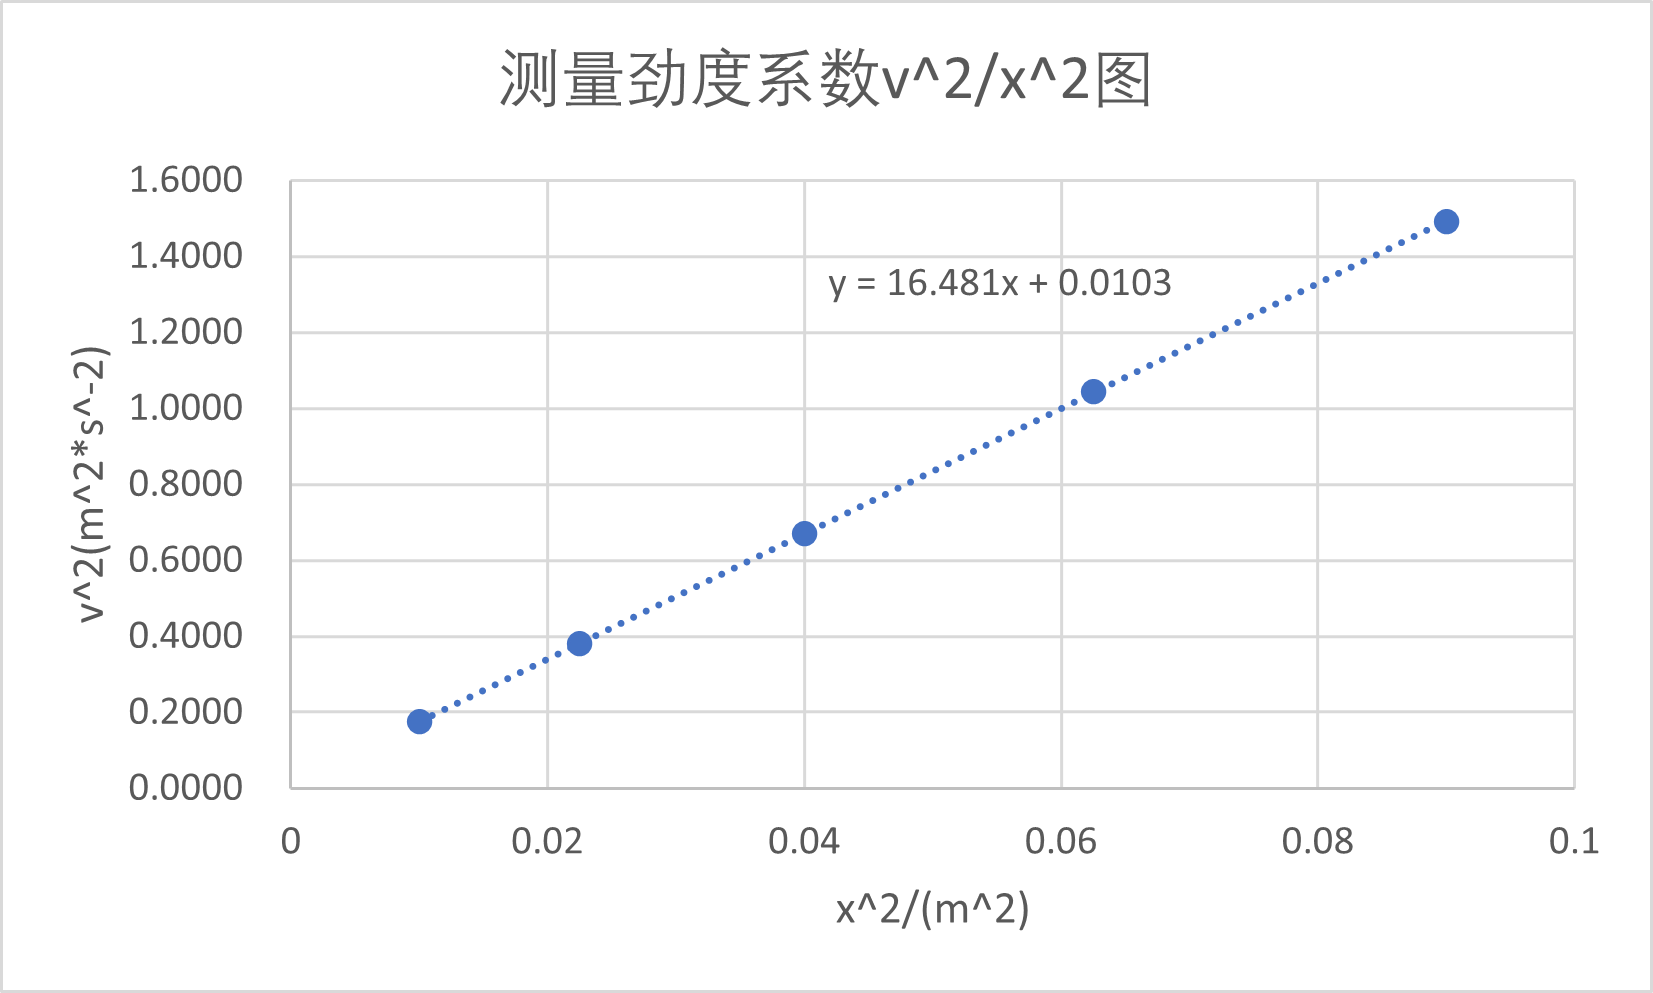
\includegraphics[width=8cm]{Fig/测量劲度系数.png}
                \caption{测量劲度系数$v^{2}/A^{2}$图}
            \end{minipage}
            \begin{minipage}[t]{0.49\linewidth}
                \centering
                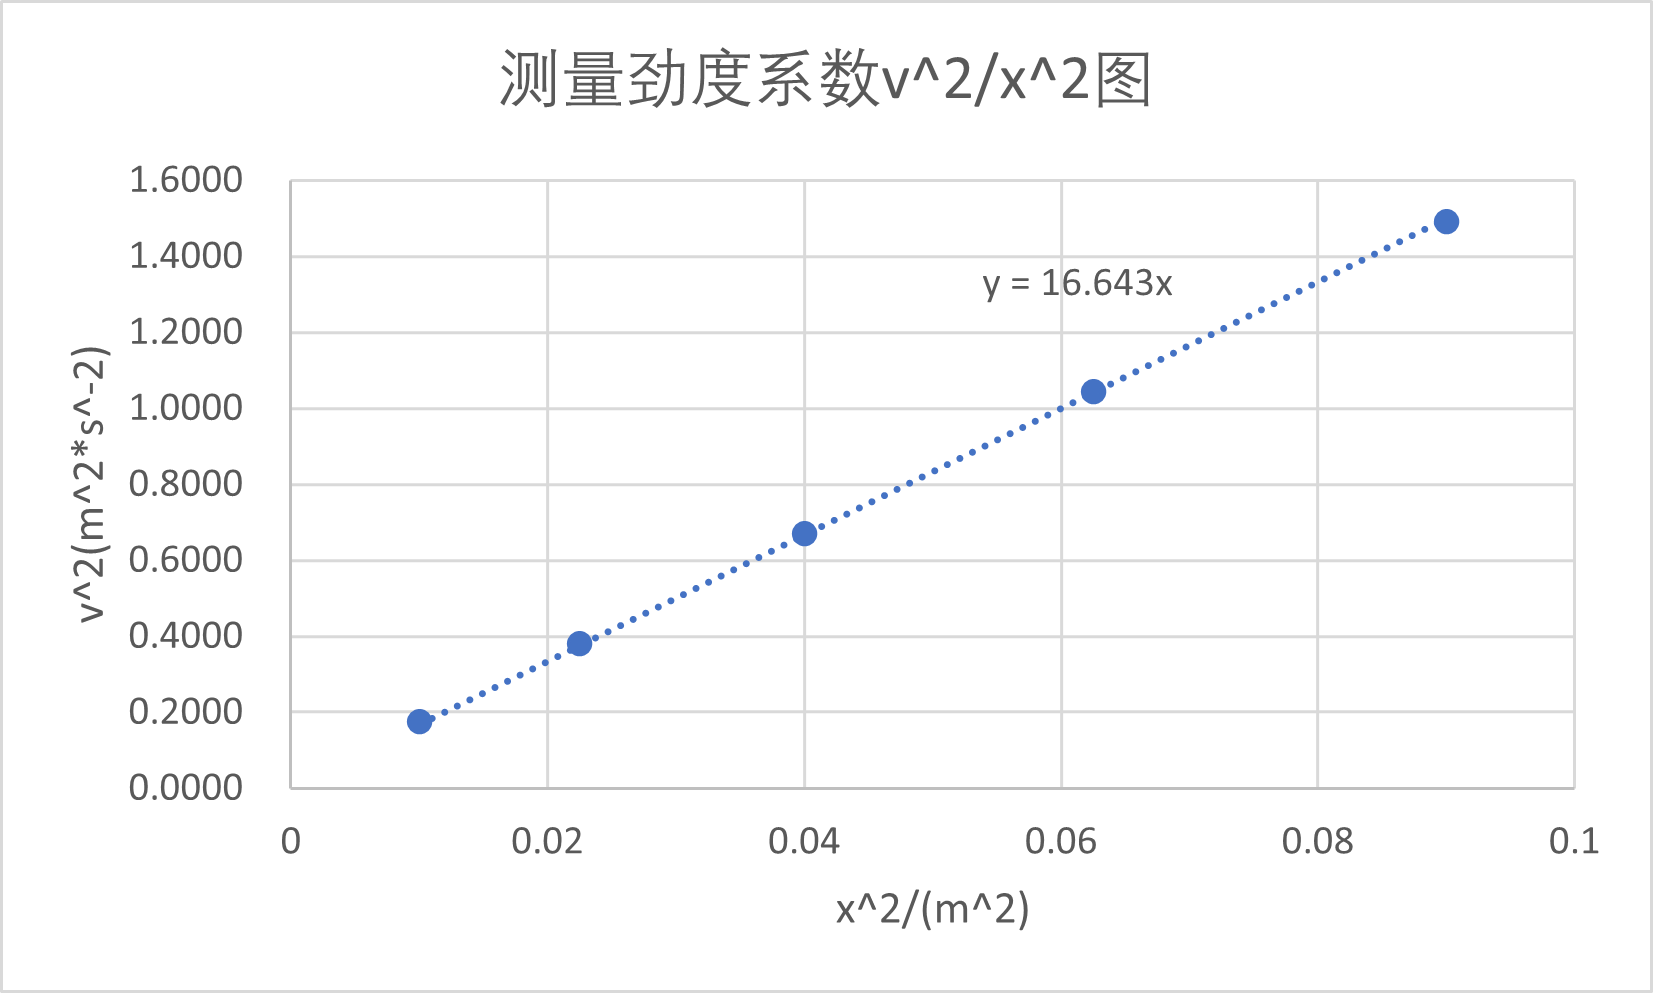
\includegraphics[width=8cm]{Fig/测量劲度系数-2.png}
                \caption{测量劲度系数$v^{2}/A^{2}$图(截距为0)}
            \end{minipage}
        \end{figure} 
    \item 数据分析
    \begin{enumerate}
        \item 由能量守恒,$\frac{1}{2}kA^{2}=\frac{1}{2}mv_{max}^2$,$v_{max}^2=\frac{k}{m_{1}+m_{0}}A^{2}$。
        \item 由4.5,$m_{1}+m_{0}=232.26g$。图像斜率$a=16.643$,得$k=a(m_{1}+m_{0})=3.866(N/m)$。
        \item 与4.4实验相比,$k$的误差为$1.1\%$,误差较小。误差来源可能为:4.7为3组数据平均值,4.4为十组数据平均值,4.4准确度更高。并且4.7无法测量等效质量,等效质量使用4.4中数据,会带来误差。
        \item 比较4.7与4.4方法,4.4测量周期,周期较长,误差更小。4.7测速度,测速误差更大。因此4.4中使用方法更好。
        \item 本实验证明了弹簧良好。
    \end{enumerate}
    
\end{enumerate}


\section{实验反思、收获与总结}
\begin{enumerate}
    \item 思考题
    \begin{enumerate}
        \item 过程中有微小阻力,会使滑块振幅不断减小。由于简谐运动周期与振幅无关,我们还可以将其看为简谐运动。若假设阻力与速度成正比,此过程为受迫振动。而空气阻力的阻尼系数较小,远远达不到临界阻尼值,因此运动形式应为振幅逐渐减小的阻尼振荡,振动周期仍旧不变。为保持滑块简谐运动,首先要调整气垫导轨水平。然后测量时尽量将振幅增大,减小阻力做功占总能量的比例。第三尽量测多组数据取平均值。
        \item 弹簧的等效质量:弹簧与滑块连接处滑块对弹簧的拉力除以重力加速度。由于弹簧一侧在导轨,另一侧在滑块,弹簧质量不完全属于滑块,因此需要测量。并且,弹簧也参与振动,也承担一部分动能。不考虑弹簧等效质量的情况下,总质量测量值小于实际值。若滑块质量较大,或弹簧质量较小,则可忽略。但是由于气垫导轨支撑力有限,滑块质量不能过大,弹簧质量/滑块质量不能小于千分之一,此部分误差无法忽略。忽略此部分误差,在4.4测量中不影响k的值,但影响4.5和4.6中计算机械能守恒时的误差。
        \item 测量周期时,光电门尽量在平衡位置上。平衡位置附近振子速度最大,振子速度大,通过光电门的时间小,误差小。光电门不在平衡位置附近会增大测量周期的误差。
        \item 气垫导轨如果不水平,在实验4.3-4.7中,重力做功,多个关键量受到影响,此时为重力与弹力两个力做功。由于无法测量重力做功量,此误差无法消除,严重影响测量准确性。但若加入恒定的重力加速度,会产生新的平衡位置,振动周期的测量不受影响。
        \item 类比实验4.1,改变两光电门距离,保持平行板前端与第一个光电门距离不变,测量两光电门距离x和滑块从进入第一个光电门到退出第二个光电门的时间差$\Delta t$,计算通过两光电门的平均速度。由$\bar{\Delta v}=\frac{\Delta x}{\Delta t}=v_{0}+\frac{a}{2} \Delta t$,作图并利用外推法可得瞬时速度$v_{0}$。
        \item 气垫导轨如果不水平,不考虑阻力的情况下,对瞬时速度的测定无影响。事实上,测定瞬时速度时,为给出恒定加速度,我们保证气垫导轨倾斜角度不变,气垫导轨必须不水平。当倾斜角度较小时,单周期下阻力影响振幅小于0.5\%,可以忽略。
        \item 若每次测量滑块和U型挡光片总质量不同,对瞬时速度测定无影响。在我们计算瞬时速度时,不需要测量滑块和U型挡光片总质量。忽略阻力时,滑块受到的加速度大小与其质量无关。在实验中,单周期下阻力影响振幅小于0.5\%,因此无需关注阻力。我们只需要保证滑块受到的加速度恒定即可。
    \end{enumerate}
    \item 个人反思
    \begin{enumerate}
        \item 释放滑块时,尽量不要给予其初速度,尽量不要使滑块与滑轨有摩擦。
        \item 实验时如果发现数据异常要及时检查仪器。我在实验中遇到实验4.7数据恒定在3.5左右的情况,重新接线后才正常。
    \end{enumerate}
\end{enumerate}

\newpage
\begin{center}
    \vspace*{1em}
    \Large \bf 第二部分\qquad 预习报告
\end{center}

\begin{enumerate}
    \item 实验原理
	\newline \hspace*{2em}简谐运动位移表达式$x=A\sin(\omega _{0}+ \phi_{0})$,周期表达式$T=2\pi \sqrt{\frac{m}{k}}$。其中$\omega _{0} = \sqrt{\frac{k}{m}}$,k为弹簧弹性系数,m为振子质量。根据三角函数的计算,可以叠加多个弹簧振子的效果。我们有$k= \frac{4\pi ^{2} m}{T^{2}}$,k与$T^{2}$成正比。由此可以拟合直线,根据斜率获取k,根据截距获取m。
	\newline \hspace*{2em}由运动轨迹的导数是其速度,简谐运动的速度也为正弦型函数,相位差$\frac{\pi}{2}$。在位移峰值,速度最小。
	\newline \hspace*{2em}由能量守恒,在弹簧振子上机械能和弹性势能不断转换。$E_{p}=\frac{1}{2} kx^{2}$,$E_{k}=\frac{1}{2} mv^{2}$。只需测量位移最大时的位移并知晓弹性系数即可计算机械能。在拥有足够精确的测速仪器下,也可以测量非位移峰值的速度从而计算机械能,以验证机械能守恒定律。
	\newline \hspace*{2em}测量速度时,我们从来不能测量瞬时速度,只能测量时间极短内的平均速度。我们知道$v_{瞬}=\lim\limits_{\delta t \to 0} \frac{\delta s}{\delta t}$。$\delta t$足够小时,认为$\bar v=\frac{\delta s}{\delta t}$。
	\newline \hspace*{2em}外推法(Extrapolation)是根据过去和现在的发展趋势推断未来的一类方法的总称,用于科技、经济和社会发展的预测,是情报研究法体系的重要部分。速度即为位移的变化趋势,用外推法可以画出图像求瞬时速度。

    \item 实验仪器
	\newline \hspace*{2em}气垫导轨下喷射出一层薄薄的气垫,使滑块不和导轨直接接触,将固体间的滑动摩擦力转化为固体和气体的滑动摩擦力,大大减小了摩擦力,对精确的测速体系很重要。电脑可以收集两光电门被挡光的时间,就此可以记录数据,作图。

\end{enumerate}
\newpage
\begin{center}
    \vspace*{1em}
    \Large \bf 第三部分\qquad 实验原始记录
\end{center}
\includepdf[pages={1-3}]{Data/实验5-数据记录表.pdf}
\end{document}